\documentclass[a4paper]{article}
\usepackage[left=2.5cm,top=2.5cm,right=2.5cm,bottom=3cm]{geometry} 
\usepackage[utf8]{inputenc}
\usepackage{graphicx} % Required for inserting images
\usepackage[table,xcdraw]{xcolor}
\usepackage{blindtext}
\usepackage{mathdots} % para el comando \iddots
\usepackage{mathrsfs} % para formato de letra
\usepackage{marvosym}
\usepackage{amsmath}
\usepackage{amsfonts}
\usepackage{amssymb}
\usepackage{listings}
\usepackage{caption}
\usepackage{float}
\usepackage{parskip}


\title{\textbf{HW8: Introduction to Financial Engineering}}
\author{Miguel Angel Aguilo Gonzalez, 1699413 \\ Judit de Paz Ramírez, 1570590 \\ Laia Mòdol Rodríguez, 1565282 \\ Elena Rubio Zabala, 1699049 \\ Guillem Tutusaus Alcaraz, 1533701 } 
\date{Diciembre 2023}

\begin{document}
\maketitle

\newpage

\section*{Ejercicio 1}
El llamado \textit{Black Monday} sigue siendo una fecha importante en la historia financiera, caracterizada por una drástica caída del -22.8\% en el rendimiento del índice S\&P500. En este informe, utilizaremos el código proporcionado en el HW2 para obtener sus datos históricos y estudiar el caso de la gran caída del S\&P500, con el mismo objetivo de lo poco predictivo que fue, pero con la principal diferencia de que ahora queremos medir su riesgo. En particular, el \textit{Black Monday} es un gran ejemplo de medición del riesgo de mercado, cuyo objetivo es saber cuánto impacto tiene la variabilidad de los activos riesgosos que forman parte de una determinada cartera.

Empezamos haciendo una gráfica de la serie temporal de los últimos dos años de datos antes del \textit{Black Monday}, pero incluyendo este último.
\begin{figure}[H]
    \centering
    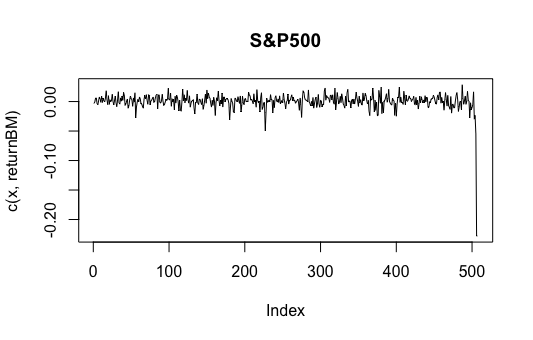
\includegraphics[width=0.6\linewidth]{plot1.png}
\end{figure}
Podemos ver que el \textit{Black Monday} fue muy inusual, se observa una drástica caída.

A continuación mostramos un histograma para los rendimientos utilizando la serie temporal hasta el \textit{Black Monday}, pero sin incluir este último. 
\begin{figure}[H]
    \centering
    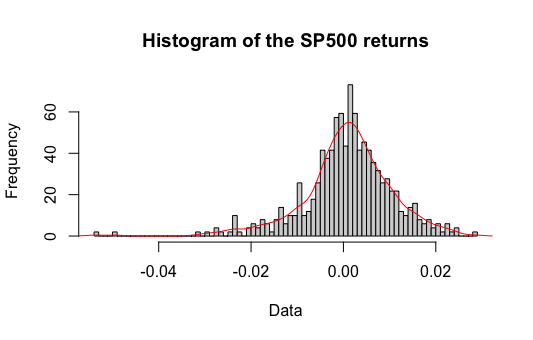
\includegraphics[width=0.6\linewidth]{plot2.png}
\end{figure}
Con el histograma observamos que estos datos parecen seguir una distribución normal centrada aproximadamente en el cero.

Con el fin de evaluar el riesgo, utilizamos una de las métricas de riesgo más tradicionales: el Valor en Riesgo (VaR). Es importante recordar que, en un horizonte temporal ($T$) y con un nivel de confianza ($\alpha$), el VaR representa la pérdida máxima que una cartera específica podría experimentar en un periodo ($T$), con una confianza del $(1-\alpha)\%$.

En nuestra evaluación, únicamente consideramos un factor de riesgo: el valor de la cartera. Por lo tanto, este factor de riesgo está directamente relacionado con el valor de la cartera a través de una función de identidad. Existen diversas metodologías para calcular el VaR; en nuestro caso, hemos decidido llevar a cabo una simulación histórica.

Dado que nuestro objetivo es calcular el Valor en Riesgo (VaR) con un nivel de confianza del 99\%, es necesario identificar el valor en el cual el 1\% de los rendimientos históricos son inferiores. Para representar esto gráficamente, hemos utilizado el histograma previo y trazado el cuantil del 1\% mediante una línea de puntos rojos.
\begin{figure}
    \centering
    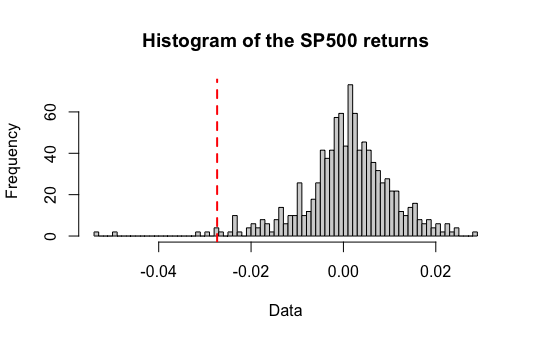
\includegraphics[width=0.6\linewidth]{plot3.png}  
\end{figure}

En concreto, a través del uso de la función \texttt{quantile()} en R, hemos obtenido un Valor en Riesgo de -0,02735.

Así pues, observamos que existe un 1\% de posibilidades de que el valor del activo disminuya un 2,7\% durante el período de un día. Recordando que la rentabilidad del \textit{Black Monday} fue del -22,8\%, está claro que el acontecimiento fue muy inesperado.

\section*{Ejercicio 2}
En este ejercicio calcularemos el valor del VaR y la cola del VaR con una confianza del 99\%. \\
Para ello, utilizaremos la 5. practica.
Extraemos el siguiente trozo de código del HW5, para hacer uso de la función que creamos del camino simple y del algoritmo de Monte Carlo para acercar el modelo:
\\
\begin{lstlisting}[language=R]
payoff_function=function(S, K) {
  return(max(K - S, 0))
}

path_sample=function(N, t0, tn, S0, r, sigma){
  x0=c() 
  x0[1]=S0 
  for(i in 1:N){
    x0[i+1]= x0[i]+r*x0[i]*((tn-t0)/N)+sigma*x0[i]*sqrt((tn-t0)/N)*rnorm(1)
  }
  return(x0)
}
\end{lstlisting}
Y adaptamos nuestra función Monte Carlo, ya que queremos calcular el VaR y su cola con un 99\% de confianza, para ello tenemos que modificar nuestra función:
\begin{lstlisting}[language=R]
monte_carlo=function(M, N, t0, tn, S0, r, sigma, payoff_function, K){
  vec=c() 
  for(i in 1:M){
    vec[i]=payoff_function(path_sample(N, t0, tn, S0, r, sigma)[N+1], K)
  }
  price=exp(r*(t0-tn))*mean(na.omit(vec)) 
  payoff=vec
  v<-numeric(M)
  for (i in 1:M){
    v[i]<-price-payoff[i]
    }
  return(v)
}
}
\end{lstlisting}
Hacemos una simulación de los precios con los datos que nos dan y creamos el histograma de simulaciones:
\begin{figure}[H]
    \centering
    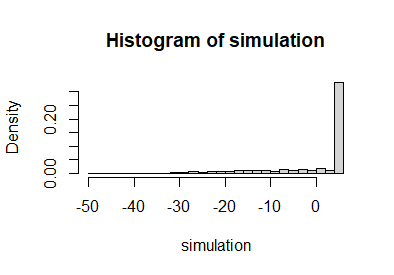
\includegraphics[width=0.6\linewidth]{Rplot111.png}  
\end{figure}
 Sabemos que tendremos los mismos parámetros que en el HW5 d), es decir, dar el precio de una opción PUT por 1 año, con una tasa de interés del 5\% y una volatilidad del 40\%. La acción cotiza actualmente a 90 EUR y la huelga de la opción PUT es 75. Una vez tenemos nuestra simulación, calculamos el VaR y lo representamos con una línea roja en el histograma, en este caso el VaR da: -35.89753
\begin{figure}[H]
    \centering
    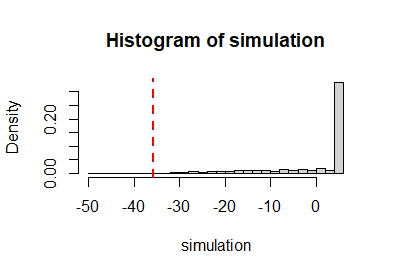
\includegraphics[width=0.6\linewidth]{Rplot112.png}  
\end{figure}
Por último,calculamos la cola del VaR, que se define como la medida de riesgo asociada con el valor en riesgo más general. Calculamos la cola de VaR como la media de los valores de simulaciones menores que el VaR, que en este caso nos da -41.52532 y la representamos con una linea azul en el histograma.
\begin{figure}[H]
    \centering
    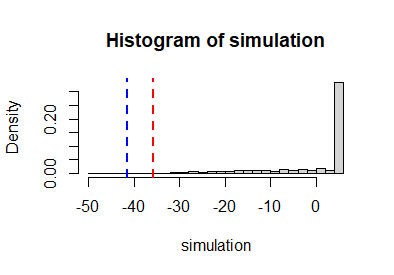
\includegraphics[width=0.6\linewidth]{Rplot113.png}
\end{figure}
\end{document}
